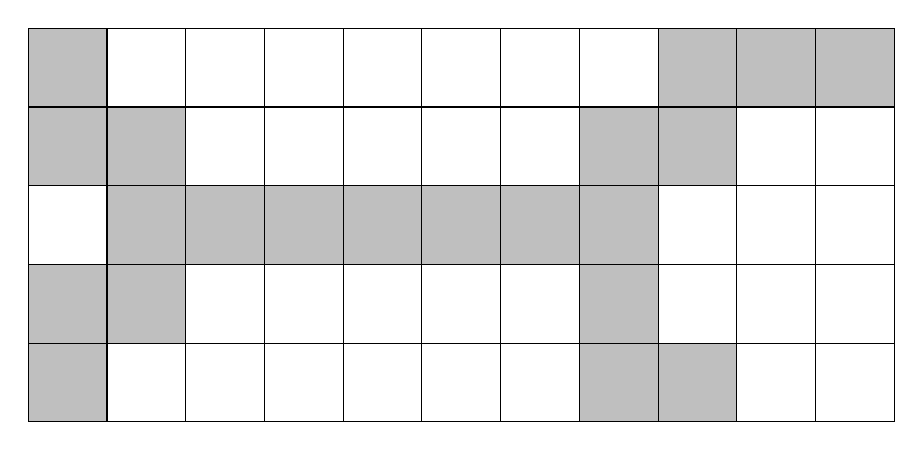
\begin{tikzpicture}
\draw[fill=lightgray] (1,3) rectangle (8,2);
\draw[fill=lightgray] (0,5) rectangle (1,4);
\draw[fill=lightgray] (0,4) rectangle (2,3);
\draw[fill=lightgray] (0,0) rectangle (1,1);
\draw[fill=lightgray] (0,1) rectangle (2,2);
\draw[fill=lightgray] (7,0) rectangle (9,1);
\draw[fill=lightgray] (7,1) rectangle (8,2);
\draw[fill=lightgray] (7,3) rectangle (9,4);
\draw[fill=lightgray] (8,4) rectangle (11,5);

\foreach \x in {0,...,11} {
\draw (\x,0) -- (\x,5);}
\foreach \y in {0,...,5} {
\draw (0,\y) -- (11,\y);}

\end{tikzpicture}